\chapter{排序算法}

\section{排序算法}

\subsection{排序算法}

应用到排序的常见比比皆是,例如当开发一个学生管理系统时需要按照学号从小到大进行排序,当开发一个电商平台时需要把同类商品按价格从低到高进行排序,当开发一款游戏时需要按照游戏得分从多到少进行排序。\\

根据时间复杂度的不同,主流的排序算法可以分为三类:

\begin{enumerate}
	\item $ O(n^2) $:冒泡排序、选择排序、插入排序
	\item $ O(nlogn) $:归并排序、快速排序、堆排序
	\item $ O(n) $:计数排序、桶排序、基数排序
\end{enumerate}

在算法界还存在着更多五花八门的排序,它们有些基于传统排序变形而来,有些则是脑洞大开,如鸡尾酒排序、猴子排序、睡眠排序等。\\

例如睡眠排序,对于待排序数组中的每一个元素,都开启一个线程,元素值是多少,就让线程睡多少毫秒。当这些线程陆续醒来的时候,睡得少的线程线性来,睡得多的线程后醒来。睡眠排序虽然挺有意思,但是没有任何实际价值。启动大量线程的资源消耗姑且不说,数值接近的元素也未必能按顺序输出,而且一旦遇到很大的元素,线程睡眠时间可能超过一个月。\\

\subsection{稳定性}

排序算法还可以根据其稳定性,划分为稳定排序和不稳定排序:

\begin{itemize}
	\item 稳定排序:值相同的元素在排序后仍然保持着排序前的顺序。
	\item 不稳定排序:值相同的元素在排序后打乱了排序前的顺序。
\end{itemize}

\begin{figure}[H]
	\centering
	\begin{tikzpicture}[font=\ttfamily,
			array/.style={matrix of nodes,nodes={draw, minimum size=10mm, fill=green!30},column sep=-\pgflinewidth, row sep=0.5mm, nodes in empty cells,
					row 1/.style={nodes={draw=none, fill=none, minimum size=5mm}},
				}]

		\draw (-4,0.7) node{原始数列};
		\draw (-3.8,-0.3) node{不稳定排序};
		\draw (-4,-1.4) node{稳定排序};

		\matrix[array] (array) {
			0 & 1 & 2                     & 3                     & 4 \\
			5 & 8 & \textcolor{orange}{6} & \textcolor{purple}{6} & 3 \\
			3 & 5 & \textcolor{purple}{6} & \textcolor{orange}{6} & 8 \\
			3 & 5 & \textcolor{orange}{6} & \textcolor{purple}{6} & 8 \\
		};
	\end{tikzpicture}
	\caption{排序稳定性}
\end{figure}

\newpage

\section{冒泡排序}

\subsection{冒泡排序(Bubble Sort)}

冒泡排序是最基础的交换排序。冒泡排序之所以叫冒泡排序,正是因为这种排序算法的每一个元素都可以像小气泡一样,根据自身大小,一点一点向着数组的一侧移动。\\

按照冒泡排序的思想,要把相邻的元素两两比较,当一个元素大于右侧相邻元素时,交换它们的位置;当一个元素小于或等于右侧相邻元素时,位置不变。\\

例如一个有8个数字组成的无序序列,进行升序排序。

\begin{figure}[H]
	\centering
	\begin{tikzpicture}[font=\ttfamily,
			array/.style={matrix of nodes,nodes={draw, minimum size=10mm, fill=green!30},column sep=-\pgflinewidth, row sep=0.5mm, nodes in empty cells,
					row 1/.style={nodes={draw=none, fill=none, minimum size=5mm}},
				}]

		\matrix[array] (array) {
			0 & 1 & 2 & 3 & 4 & 5 & 6 & 7 \\
			5 & 8 & 6 & 3 & 9 & 2 & 1 & 7 \\
			5 & 8 & 6 & 3 & 9 & 2 & 1 & 7 \\
			5 & 6 & 8 & 3 & 9 & 2 & 1 & 7 \\
			5 & 6 & 3 & 8 & 9 & 2 & 1 & 7 \\
			5 & 6 & 3 & 8 & 9 & 2 & 1 & 7 \\
			5 & 6 & 3 & 8 & 2 & 9 & 1 & 7 \\
			5 & 6 & 3 & 8 & 2 & 1 & 9 & 7 \\
			5 & 6 & 3 & 8 & 2 & 1 & 7 & 9 \\
		};

		\draw[-, very thick, red] (-4,3.95) rectangle (-2,2.95);
		\draw[-, very thick, red] (-3,2.85) rectangle (-1,1.89);
		\draw[-, very thick, red] (-2,1.8) rectangle (0,0.79);
		\draw[-, very thick, red] (-1,0.71) rectangle (1,-0.25);
		\draw[-, very thick, red] (0,-0.35) rectangle (2,-1.33);
		\draw[-, very thick, red] (1,-1.39) rectangle (3,-2.4);
		\draw[-, very thick, red] (2,-2.49) rectangle (4,-3.47);

		\draw[<->, very thick, red] (-2.4,2.4) -- (-1.6,2.4);
		\draw[<->, very thick, red] (-1.35,1.3) -- (-0.6,1.3);
		\draw[<->, very thick, red] (0.6,-0.8) -- (1.4,-0.8);
		\draw[<->, very thick, red] (1.65,-1.9) -- (2.4,-1.9);
		\draw[<->, very thick, red] (2.65,-2.95) -- (3.4,-2.95);

		\draw[-, very thick, blue] (3,-3.55) rectangle (4,-4.55);
	\end{tikzpicture}
	\caption{冒泡排序第1轮}
\end{figure}

这样一来,元素9作为数列中最大的元素,就像是汽水里的小气泡一样,浮到了最右侧。这时,冒泡排序的第1轮就结束了。数列最右侧元素9的位置可以认为是一个有序区域,有序区域目前只有1个元素。\\

接着进行第2轮排序:

\begin{figure}[H]
	\centering
	\begin{tikzpicture}[font=\ttfamily,
			array/.style={matrix of nodes,nodes={draw, minimum size=10mm, fill=green!30},column sep=-\pgflinewidth, row sep=0.5mm, nodes in empty cells,
					row 1/.style={nodes={draw=none, fill=none, minimum size=5mm}},
				}]

		\matrix[array] (array) {
			0 & 1 & 2 & 3 & 4 & 5 & 6 & 7 \\
			5 & 6 & 3 & 8 & 2 & 1 & 7 & 9 \\
			5 & 6 & 3 & 8 & 2 & 1 & 7 & 9 \\
			5 & 3 & 6 & 8 & 2 & 1 & 7 & 9 \\
			5 & 3 & 6 & 8 & 2 & 1 & 7 & 9 \\
			5 & 3 & 6 & 2 & 8 & 1 & 7 & 9 \\
			5 & 3 & 6 & 2 & 1 & 8 & 7 & 9 \\
			5 & 3 & 6 & 2 & 1 & 7 & 8 & 9 \\
		};

		\draw[-, very thick, red] (-4,3.4) rectangle (-2,2.4);
		\draw[-, very thick, red] (-3,2.3) rectangle (-1,1.37);
		\draw[-, very thick, red] (-2,1.27) rectangle (0,0.29);
		\draw[-, very thick, red] (-1,0.2) rectangle (1,-0.77);
		\draw[-, very thick, red] (0,-0.86) rectangle (2,-1.84);
		\draw[-, very thick, red] (1,-1.92) rectangle (3,-2.9);

		\draw[<->, very thick, red] (-2.4,1.85) -- (-1.6,1.85);
		\draw[<->, very thick, red] (-0.4,-0.3) -- (0.4,-0.3);
		\draw[<->, very thick, red] (0.6,-1.35) -- (1.4,-1.35);
		\draw[<->, very thick, red] (1.6,-2.4) -- (2.4,-2.4);

		\draw[-, very thick, blue] (3,3.4) rectangle (4,2.4);
		\draw[-, very thick, blue] (3,2.32) rectangle (4,1.33);
		\draw[-, very thick, blue] (3,1.25) rectangle (4,0.26);
		\draw[-, very thick, blue] (3,0.2) rectangle (4,-0.8);
		\draw[-, very thick, blue] (3,-0.9) rectangle (4,-1.85);
		\draw[-, very thick, blue] (3,-1.95) rectangle (4,-2.9);
		\draw[-, very thick, blue] (2,-3) rectangle (4,-4);
	\end{tikzpicture}
	\caption{冒泡排序第2轮}
\end{figure}

第2轮排序结束后,数列右侧的有序区有了2个元素。\\

根据相同的方法,完成剩下的排序:

\begin{figure}[H]
	\centering
	\begin{tikzpicture}[font=\ttfamily,
			array/.style={matrix of nodes,nodes={draw, minimum size=10mm, fill=green!30},column sep=-\pgflinewidth, row sep=0.5mm, nodes in empty cells,
					row 1/.style={nodes={draw=none, fill=none, minimum size=5mm}},
				}]

		\matrix[array] (array) {
			0 & 1 & 2 & 3 & 4 & 5 & 6 & 7 \\
			3 & 5 & 2 & 1 & 6 & 7 & 8 & 9 \\
			3 & 2 & 1 & 5 & 6 & 7 & 8 & 9 \\
			2 & 1 & 3 & 5 & 6 & 7 & 8 & 9 \\
			1 & 2 & 3 & 5 & 6 & 7 & 8 & 9 \\
			1 & 2 & 3 & 5 & 6 & 7 & 8 & 9 \\
		};

		\draw (-5,1.9) node{第3轮};
		\draw (-5,0.8) node{第4轮};
		\draw (-5,-0.3) node{第5轮};
		\draw (-5,-1.4) node{第6轮};
		\draw (-5,-2.4) node{第7轮};

		\draw[-, very thick, blue] (1,2.32) rectangle (4,1.33);
		\draw[-, very thick, blue] (0,1.25) rectangle (4,0.26);
		\draw[-, very thick, blue] (-1,0.2) rectangle (4,-0.8);
		\draw[-, very thick, blue] (-2,-0.9) rectangle (4,-1.85);
		\draw[-, very thick, blue] (-3,-1.95) rectangle (4,-2.9);
	\end{tikzpicture}
	\caption{冒泡排序第3 $ \sim $ 7轮}
\end{figure}

\vspace{0.5cm}

\subsection{算法分析}

冒泡排序是一种稳定排序,值相等的元素并不会打乱原本的顺序。由于该排序算法的每一轮都要遍历所有元素,总共遍历n - 1轮。

\begin{table}[H]
	\centering
	\setlength{\tabcolsep}{5mm}{
		\begin{tabular}{|c|c|c|c|}
			\hline
			\textbf{时间复杂度} & \textbf{空间复杂度} & \textbf{稳定性} & \textbf{设计思想} \\
			\hline
			$ O(n^2) $          & $ O(1) $            & 稳定            & 贪心法            \\
			\hline
		\end{tabular}
	}
	\caption{冒泡排序算法分析}
\end{table}

\mybox{冒泡排序}

\begin{lstlisting}[language=C++]
int *bubble_sort(int *arr, int n) {
	for (int i = 0; i < n; i++) {
		for (int j = 0; j < n - i - 1; j++) {
			if (arr[j] > arr[j + 1]) {
				swap(arr[j], arr[j + 1]);
			}
		}
	}
	return arr;
}
\end{lstlisting}

\vspace{0.5cm}

\mybox{逆序对}\\

假设数组有n个元素,如果A[i] > A[j], i < j,那么A[i]和A[j]就被称为逆序对(inversion)。

\begin{lstlisting}[language=C++]
int count_inverses(int *arr, int n) {
	int count = 0;
	for (int i = 0; i < n; i++) {
		for (int j = i + 1; j < n; j++) {
			if (arr[i] > arr[j]) {
				count++;
			}
		}
	}
	return count;
}
\end{lstlisting}

\vspace{0.5cm}

\subsection{冒泡排序第一次优化}

常规的冒泡排序需要进行n - 1轮循环,即使在中途数组已经有序,但是还是会继续剩下的循环。例如当数组是\{2, 1, 3, 4, 5\}时,在经过一轮排序后已经变为有序状态,再进行多余的循环就会浪费时间。\\

为了解决这个问题,可以在每一轮循环中设置一个标志。如果该轮循环中有元素发生过交换,那么就有必要进行下一轮循环。如果没有发生过交换,说明当前数组已经完成排序。\\

\mybox{冒泡排序第一次优化}

\begin{lstlisting}[language=C++]
int *bubble_sort(int *arr, int n) {
	for (int i = 0; i < n; i++) {
		bool swapped = false;
		for (int j = 0; j < n - i - 1; j++) {
			if (arr[j] > arr[j + 1]) {
				swap(arr[j], arr[j + 1]);
				swapped = true;
			}
		}
		if (!swapped) {
			break;
		}
	}

	return arr;
}
\end{lstlisting}

\vspace{0.5cm}

\subsection{冒泡排序第二次优化}

在经过一次优化后,算法还存在一个问题,例如数组\{2, 3, 1, 4, 5, 6\}在经过一轮交换后变为\{2, 1, 3, 4, 5, 6\},但是在下一轮时后面有很多次比较都是多余的,因为并没有产生交换操作。\\

为了解决这个问题,可以再设置一个标志位,用于记录当前轮所交换的最后一个元素的下标。在下一轮排序中,只需比较到该标志位即可,因此之后的元素在上一轮中没有交换过,在这一轮中也不可能交换了。\\

\mybox{冒泡排序第二次优化}

\begin{lstlisting}[language=C++]
int *bubble_sort(int *arr, int n) {
	int right = n - 1;
	for (int i = 0; i < n; i++) {
		bool swapped = false;
		int last = 0;
		for (int j = 0; j < right; j++) {
			if (arr[j] > arr[j + 1]) {
				swap(arr[j], arr[j + 1]);
				swapped = true;
				last = j;
			}
		}
		if (!swapped) {
			break;
		}
		right = last;
	}

	return arr;
}
\end{lstlisting}

\newpage

\section{选择排序}

\subsection{选择排序(Selection Sort)}

有了冒泡排序为什么还要发明选择排序?冒泡排序有个很大的弊端,就是元素交换次数太多了。\\

想象一个场景,假设你是一名体育老师,正在指挥一群小学生按照个头从矮到高的顺序排队。采用冒泡排序的方法需要频繁交换相邻学生的位置,同学们心里恐怕会想:“这体育老师是不是有毛病啊?”\\

在程序运行的世界里,虽然计算机并不会产生什么负面情绪,但是频繁的数组元素交换意味着更多的内存读写操作,严重影响了代码运行效率。\\

有一个简单的办法,就是每一次找到个子最矮的学生,直接交换到队伍的前面。\\

例如一个有8个数字组成的无序序列,进行升序排序。

\begin{figure}[H]
	\centering
	\begin{tikzpicture}[font=\ttfamily,
			array/.style={matrix of nodes,nodes={draw, minimum size=10mm, fill=green!30},column sep=-\pgflinewidth, row sep=0.5mm, nodes in empty cells,
					row 1/.style={nodes={draw=none, fill=none, minimum size=5mm}},
				}]

		\matrix[array] (array) {
			0 & 1 & 2 & 3 & 4 & 5 & 6 & 7 \\
			5 & 8 & 6 & 3 & 9 & 2 & 1 & 7 \\
			1 & 8 & 6 & 3 & 9 & 2 & 5 & 7 \\
			1 & 2 & 6 & 3 & 9 & 8 & 5 & 7 \\
			1 & 2 & 3 & 6 & 9 & 8 & 5 & 7 \\
			1 & 2 & 3 & 5 & 9 & 8 & 6 & 7 \\
			1 & 2 & 3 & 5 & 6 & 8 & 9 & 7 \\
			1 & 2 & 3 & 5 & 6 & 7 & 9 & 8 \\
			1 & 2 & 3 & 5 & 6 & 7 & 8 & 9 \\
		};

		\draw (-5,3.4) node{原数组};
		\draw (-5,2.4) node{第1轮};
		\draw (-5,1.3) node{第2轮};
		\draw (-5,0.2) node{第3轮};
		\draw (-5,-0.9) node{第4轮};
		\draw (-5,-1.9) node{第5轮};
		\draw (-5,-3) node{第6轮};
		\draw (-5,-4) node{第7轮};

		\draw[-, very thick, blue] (-4,2.85) rectangle (-3,1.9);
		\draw[-, very thick, blue] (-4,1.8) rectangle (-2,0.8);
		\draw[-, very thick, blue] (-4,0.7) rectangle (-1,-0.25);
		\draw[-, very thick, blue] (-4,-0.35) rectangle (0,-1.3);
		\draw[-, very thick, blue] (-4,-1.4) rectangle (1,-2.4);
		\draw[-, very thick, blue] (-4,-2.5) rectangle (2,-3.45);
		\draw[-, very thick, blue] (-4,-3.55) rectangle (3,-4.5);
	\end{tikzpicture}
	\caption{选择排序}
\end{figure}

\vspace{0.5cm}

\subsection{算法分析}

算法每一轮选出最小值,再交换到左侧的时间复杂度是$ O(n) $,一共迭代n - 1轮,总的时间复杂度是$ O(n^2) $。\\

由于算法所做的是原地排序,并没有利用额外的数据结构,所以空间复杂度是$ O(1) $。

\begin{table}[H]
	\centering
	\setlength{\tabcolsep}{5mm}{
		\begin{tabular}{|c|c|c|c|}
			\hline
			\textbf{时间复杂度} & \textbf{空间复杂度} & \textbf{稳定性} & \textbf{设计思想} \\
			\hline
			$ O(n^2) $          & $ O(1) $            & 不稳定          & 减治法            \\
			\hline
		\end{tabular}
	}
	\caption{选择排序算法分析}
\end{table}

\mybox{选择排序}

\begin{lstlisting}[language=C++]
int* selection_sort(int* arr, int n) {
	for (int i = 0; i < n - 1; i++) {
		int minIndex = i;
		for (int j = i + 1; j < n; j++) {
			if (arr[j] < arr[minIndex]) {
				minIndex = j;
			}
		}
		swap(arr[i], arr[minIndex]);
	}

	return arr;
}
\end{lstlisting}

\vspace{0.5cm}

\subsection{选择排序优化}

选择排序的整体思想是在一个序列当中选出一个最小的元素,和第一个元素交换,然后在剩下的找最小的,和第二个元素交换。这样最终就可以得到一个有序序列。但是为了更加高效,可以每次选择出一个最小值和一个最大值,分别放在序列的最左和最右边。\\

\mybox{选择排序优化}

\begin{lstlisting}[language=C++]
int* selection_sort(int* arr, int n) {
	for (int i = 0; i < n / 2; i++) {
		int minIndex = i;
		int maxIndex = n - i - 1;

		for (int j = i; j < n - i; j++) {
			if (arr[j] < arr[minIndex]) {
				minIndex = j;
			}
			if (arr[j] > arr[maxIndex]) {
				maxIndex = j;
			}
		}

		swap(arr[i], arr[minIndex]);

		// In case of i == maxIndex before swap(arr[i], arr[minIndex]), it's now at minIndex.
		if (i == maxIndex) {
			maxIndex = minIndex;
		}

		swap(arr[n - i - 1], arr[maxIndex]);
	}

	return arr;
}
\end{lstlisting}

\newpage

\section{插入排序}

\subsection{插入排序(Insertion Sort)}

如何对扑克牌进行排序呢?例如现在手上有红桃6, 7, 9, 10这四张牌,已经处于升序排序状态。这时候抓到了一张红桃8,如何让手上的五张牌重新变成升序呢?\\

使用冒泡排序?选择排序?恐怕正常人打牌的时候都不会那么做。最自然最简单的方式,是在已经有序的四张牌中找到红桃8应该插入的位置,也就是7和9之间,把红桃8插入进去。

\begin{figure}[H]
	\centering
	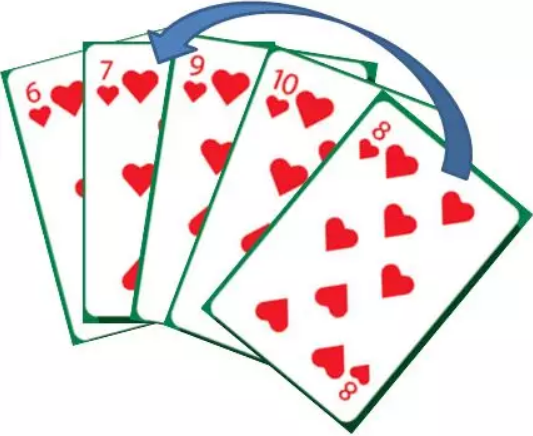
\includegraphics[scale=0.4]{img/Chapter8/8-4/1.png}
\end{figure}

例如一个有8个数字组成的无序序列,进行升序排序。

\begin{figure}[H]
	\centering
	\begin{tikzpicture}[font=\ttfamily,
			array/.style={matrix of nodes,nodes={draw, minimum size=10mm, fill=green!30},column sep=-\pgflinewidth, row sep=0.5mm, nodes in empty cells,
					row 1/.style={nodes={draw=none, fill=none, minimum size=5mm}},
				}]

		\matrix[array] (array) {
			0 & 1 & 2 & 3 & 4 & 5 & 6 & 7 \\
			5 & 8 & 6 & 3 & 9 & 2 & 1 & 7 \\
			5 & 8 & 6 & 3 & 9 & 2 & 1 & 7 \\
			5 & 6 & 8 & 3 & 9 & 2 & 1 & 7 \\
			3 & 5 & 6 & 8 & 9 & 2 & 1 & 7 \\
			3 & 5 & 6 & 8 & 9 & 2 & 1 & 7 \\
			2 & 3 & 5 & 6 & 8 & 9 & 1 & 7 \\
			1 & 2 & 3 & 5 & 6 & 8 & 9 & 7 \\
			1 & 2 & 3 & 5 & 6 & 7 & 8 & 9 \\
		};

		\draw (-5,3.4) node{原数组};
		\draw (-5,2.4) node{第1轮};
		\draw (-5,1.3) node{第2轮};
		\draw (-5,0.2) node{第3轮};
		\draw (-5,-0.9) node{第4轮};
		\draw (-5,-1.9) node{第5轮};
		\draw (-5,-3) node{第6轮};
		\draw (-5,-4) node{第7轮};

		\draw[-, very thick, blue] (-4,3.9) rectangle (-3,2.95);
		\draw[-, very thick, blue] (-4,2.85) rectangle (-2,1.9);
		\draw[-, very thick, blue] (-4,1.8) rectangle (-1,0.8);
		\draw[-, very thick, blue] (-4,0.7) rectangle (0,-0.25);
		\draw[-, very thick, blue] (-4,-0.35) rectangle (1,-1.3);
		\draw[-, very thick, blue] (-4,-1.4) rectangle (2,-2.4);
		\draw[-, very thick, blue] (-4,-2.5) rectangle (3,-3.45);
		\draw[-, very thick, blue] (-4,-3.55) rectangle (4,-4.5);
	\end{tikzpicture}
	\caption{插入排序}
\end{figure}

\vspace{0.5cm}

\subsection{算法分析}

插入排序要进行n - 1轮,每一轮在最坏情况下的比较复制次数分别是1次、2次、3次、4次...一直到n - 1次,所以最坏时间复杂度是$ O(n^2) $。\\

至于空间复杂度,由于插入排序是在原地进行排序,并没有引入额外的数据结构,所以空间复杂度是$ O(1) $。

\begin{table}[H]
	\centering
	\setlength{\tabcolsep}{5mm}{
		\begin{tabular}{|c|c|c|c|}
			\hline
			\textbf{时间复杂度} & \textbf{空间复杂度} & \textbf{稳定性} & \textbf{设计思想} \\
			\hline
			$ O(n^2) $          & $ O(1) $            & 稳定            & 减治法            \\
			\hline
		\end{tabular}
	}
	\caption{插入排序算法分析}
\end{table}

\mybox{插入排序}

\begin{lstlisting}[language=Java]
public static int[] insertionSort(int[] arr) {
	for (int i = 1; i < arr.length; i++) {
		int temp = arr[i];
		int j = i - 1;
		while (j >= 0 && temp < arr[j]) {
			arr[j + 1] = arr[j];
			j--;
		}
		arr[j + 1] = temp;
	}

	return arr;
}
\end{lstlisting}

\vspace{0.5cm}

\subsection{折半插入排序(Binary Insertion Sort)}

折半插入排序是对插入排序的改进,其过程就是不断依次将元素插入前面已经排好序的序列中,在寻找插入点时采用了折半查找。\\

\mybox{折半插入排序}

\begin{lstlisting}[language=Java]
public static int[] insertionSort(int[] arr) {
	for (int i = 1; i < arr.length; i++) {
		int temp = arr[i];
		int left = 0;
		int right = i - 1;

		while (left <= right) {
			int mid = (left + right) / 2;
			if (temp < arr[mid]) {
				right = mid - 1;
			} else {
				left = mid + 1;
			}
		}

		for (int j = i - 1; j >= left; j--) {
			arr[j + 1] = arr[j];
		}
		arr[left] = temp;
	}

	return arr;
}
\end{lstlisting}

\newpage

\section{希尔排序}

\subsection{希尔排序(Shell Sort)}

希尔排序本质上是直接插入排序的升级版。对于插入排序而言,在大多数元素已经有序的情况下,工作量会比较小。这个结论很明显,如果一个数组大部分元素都有序,那么数组中的元素自然不需要频繁地进行比较和交换。\\

如何能够让待排序的数组中大部分元素有序呢?需要对原始数组进行预处理,使得原始数组的大部分元素变得有序。采用分组的方法,可以将数组进行一定程度地粗略调整。\\

例如一个有8个数字组成的无序序列\{5, 8, 6, 3, 9, 2, 1, 7\},进行升序排序。让元素两两一组,同组两个元素之间的跨度为数组总长度的一半。\\

接着让每组元素进行独立排序,排序方式使用直接插入排序即可。由于每一组的元素数量很少,所以插入排序的工作量很少。这样一来,仅仅经过几次简单的交换,数组整体的有序程序得到了显著提高,使得后续再进行直接插入排序的工作量大大减少。\\

但是这样还不算完,还可以进一步缩小分组跨度,重复上述工作。\\

例如一个有8个数字组成的无序序列\{5, 8, 6, 3, 9, 2, 1, 7\},进行升序排序。

\begin{figure}[H]
	\centering
	\begin{tikzpicture}[font=\ttfamily,
			array/.style={matrix of nodes,nodes={draw, minimum size=10mm, fill=green!30},column sep=-\pgflinewidth, row sep=0.5mm, nodes in empty cells,
					row 1/.style={nodes={draw=none, fill=none, minimum size=5mm}},
				}]

		\matrix[array] (array) {
			0 & 1 & 2 & 3 & 4 & 5 & 6 & 7 \\
			5 & 2 & 1 & 3 & 9 & 8 & 6 & 7 \\
		};

		\draw[-, red] (-3.5,-0.8) -- (-3.5,-1.2) -- (0.5,-1.2) -- (0.5,-0.8);
		\draw[-, red] (-2.5,-0.8) -- (-2.5,-1.4) -- (1.5,-1.4) -- (1.5,-0.8);
		\draw[-, red] (-1.5,-0.8) -- (-1.5,-1.6) -- (2.5,-1.6) -- (2.5,-0.8);
		\draw[-, red] (-0.5,-0.8) -- (-0.5,-1.8) -- (3.5,-1.8) -- (3.5,-0.8);
	\end{tikzpicture}
	\caption{跨度为4分组交换}
\end{figure}

\begin{figure}[H]
	\centering
	\begin{tikzpicture}[font=\ttfamily,
			array/.style={matrix of nodes,nodes={draw, minimum size=10mm, fill=green!30},column sep=-\pgflinewidth, row sep=0.5mm, nodes in empty cells,
					row 1/.style={nodes={draw=none, fill=none, minimum size=5mm}},
				}]

		\matrix[array] (array) {
			0 & 1 & 2 & 3 & 4 & 5 & 6 & 7 \\
			1 & 2 & 5 & 3 & 6 & 7 & 9 & 8 \\
		};

		\draw[-, red] (-3.5,-0.8) -- (-3.5,-1.2) -- (-1.6,-1.2) -- (-1.6,-0.8);
		\draw[-, red] (-2.5,-0.8) -- (-2.5,-1.4) -- (-0.6,-1.4) -- (-0.6,-0.8);
		\draw[-, red] (-1.5,-0.8) -- (-1.5,-1.6) -- (0.4,-1.6) -- (0.4,-0.8);
		\draw[-, red] (-0.5,-0.8) -- (-0.5,-1.2) -- (1.4,-1.2) -- (1.4,-0.8);
		\draw[-, red] (0.5,-0.8) -- (0.5,-1.4) -- (2.5,-1.4) -- (2.5,-0.8);
		\draw[-, red] (1.5,-0.8) -- (1.5,-1.6) -- (3.5,-1.6) -- (3.5,-0.8);
	\end{tikzpicture}
	\caption{跨度为2分组交换}
\end{figure}

\begin{figure}[H]
	\centering
	\begin{tikzpicture}[font=\ttfamily,
			array/.style={matrix of nodes,nodes={draw, minimum size=10mm, fill=green!30},column sep=-\pgflinewidth, row sep=0.5mm, nodes in empty cells,
					row 1/.style={nodes={draw=none, fill=none, minimum size=5mm}},
				}]

		\matrix[array] (array) {
			0 & 1 & 2 & 3 & 4 & 5 & 6 & 7 \\
			1 & 2 & 3 & 5 & 6 & 7 & 8 & 9 \\
		};
	\end{tikzpicture}
	\caption{跨度为1分组交换}
\end{figure}

希尔排序的发明者是计算机科学家Donald Shell。希尔排序中说使用的分组跨度被称为希尔排序的增量。增量的选择可以有很多种,最朴素的就是Donald Shell在发明希尔排序时所提出的逐步折半的方法。\\

\subsection{算法分析}

希尔排序利用分组粗略调整的方式减少了直接插入排序的工作量,使得算法的平均时间复杂度低于$ O(n^2) $。但是在某些极端情况下,希尔排序的最坏时间复杂度仍然是$ O(n^2) $,甚至比插入排序更慢。\\

例如\{2, 1, 5, 3, 7, 6, 9, 8\},无论是以4为增量,还是以2为增量,每组内部的元素都没有任何交换。直到增量缩减为1,数组才会按照直接插入排序的方式进行调整。\\

对于这样的数组,希尔排序不但没有减少直接插入排序的工作量,反而白白增加了分组操作的成本。\\

这是因为每一轮希尔增量之间都是等比的,这就导致了希尔增量存在盲区。为了避免这样的极端情况,科学家发明了许多更为严谨的增量方式。其中最具有代表性的是Hibbard增量和Sedgewick增量。

\subsubsection{Hibbard增量序列}

Hibbard增量序列为$ 1, 3, 7, 15, \dots $,通项公式为$ 2^i - 1 $。\\

利用这种增量方式的希尔排序,最坏时间复杂度是$ O(n^{3/2}) $。\\

\subsubsection{Sedgewick增量序列}

Sedgewick增量序列为$ 1, 5, 19, 41, 109, \dots $,通项公式为$ 9 \times 4^i - 9 \times 2^i + 1 $和$ 4^{i+2} - 3 \times 2^{i+2} + 1 $。\\

利用这种增量方式的希尔排序,最坏时间复杂度是$ O(n^{4/3}) $。\\

这两种增量方式的时间复杂度需要很复杂的数学证明,有些是人们的大致猜想。

\begin{table}[H]
	\centering
	\setlength{\tabcolsep}{5mm}{
		\begin{tabular}{|c|c|c|}
			\hline
			\textbf{时间复杂度}   & \textbf{空间复杂度} & \textbf{稳定性} \\
			\hline
			$ O(n^{1.3 \sim 2}) $ & $ O(1) $            & 不稳定          \\
			\hline
		\end{tabular}
	}
	\caption{希尔排序算法分析}
\end{table}

\newpage

\section{归并排序}

\subsection{归并排序(Merge Sort)}

归并排序算法采用分治法:

\begin{enumerate}
	\item 分解:将序列每次折半划分。
	\item 合并:将划分后的序列两两按序合并。
\end{enumerate}

\begin{figure}[H]
	\centering
	\begin{tikzpicture}[level distance=1.2cm,
			level 1/.style={sibling distance=4cm},
			level 2/.style={sibling distance=2cm},
			level 3/.style={sibling distance=1cm},
			edgedown/.style={edge from parent/.style={draw=red,thick,-latex}},
			edgeup/.style={edge from parent/.style={draw=green!50!black,thick,latex-}}
		]

		\node[gblock=7,yshift=-7.2cm] (A') {3 \nodepart{two} 9 \nodepart{three} 10 \nodepart{four} 27 \nodepart{five} 39 \nodepart{six}43 \nodepart{seven}82}
		[grow=up,edgeup]
		child {node[gblock=3] (B2') {9 \nodepart{two} 10 \nodepart{three} 82}
				child {node[gblock=1] (C4') {10}
						child {node[gblock=1] (D7') {10}}
					}
				child {node[gblock=2] (C2') {9 \nodepart{two} 82}
						child {node[gblock=1] (D3') {82}}
						child {node[gblock=1] (D4') {9}}
					}
			}
		child {node[gblock=4] (B1') {3 \nodepart{two} 27 \nodepart{three} 39 \nodepart{four} 43}
				child {node[gblock=2] (C3') {3 \nodepart{two} 43}
						child {node[gblock=1] (D5') {3}}
						child {node[gblock=1] (D6') {43}}
					}
				child {node[gblock=2] (C1') {27 \nodepart{two} 39}
						child {node[gblock=1] (D1') {27}}
						child {node[gblock=1] (D2') {39}}
					}
			};

		\node[block=7] (A) {39 \nodepart{two} 27 \nodepart{three} 43 \nodepart{four} 3 \nodepart{five} 9 \nodepart{six}82 \nodepart{seven}10}
		[grow=down,edgedown]
		child {node[block=4] (B1) {39 \nodepart{two} 27 \nodepart{three} 43 \nodepart{four} 3}
				child {node[block=2] (C1) {39 \nodepart{two} 27}
						child {node[block=1] (D1) {39}}
						child {node[block=1] (D2) {27}}
					}
				child {node[block=2] (C2) {43 \nodepart{two} 3}
						child {node[block=1] (D3) {43}}
						child {node[block=1] (D4) {3}}
					}
			}
		child {node[block=3] (B2) {9 \nodepart{two} 82 \nodepart{three} 10}
				child {node[block=2] (C3) {9 \nodepart{two} 82}
						child {node[block=1] (D5) {9}}
						child {node[block=1] (D6) {82}}
					}
				child {node[block=1] (C4) {10}
						child {node[block=1] (D7) {10}}
					}
			};
	\end{tikzpicture}
	\caption{归并排序}
\end{figure}

归并排序每次将数组折半对分,一共分了$ logn $次,每一层进行合并操作的运算量是n,所以时间复杂度为$ O(nlogn) $。归并排序的速度仅次于快速排序。\\

\begin{table}[H]
	\centering
	\setlength{\tabcolsep}{5mm}{
		\begin{tabular}{|c|c|c|c|}
			\hline
			\textbf{时间复杂度} & \textbf{空间复杂度} & \textbf{稳定性} & \textbf{设计思想} \\
			\hline
			$ O(nlogn) $        & $ O(n) $            & 稳定            & 分治法            \\
			\hline
		\end{tabular}
	}
	\caption{归并排序算法分析}
\end{table}

\mybox{归并排序}

\begin{lstlisting}[language=Python]
def merge_sort(lst):
    """Merge Sort (original v1.0)"""
    if len(lst) <= 1:
        return lst
    
    mid = len(lst) // 2
    left_half = lst[:mid]
    right_half = lst[mid:]

    merge_sort(left_half)
    merge_sort(right_half)

    i = 0
    j = 0
    k = 0

    while i < len(left_half) and j < len(right_half):
        if left_half[i] < right_half[j]:
            lst[k] = left_half[i]
            i += 1
        else:
            lst[k] = right_half[j]
            j += 1
        k += 1
    
    while i < len(left_half):
        lst[k] = left_half[i]
        i += 1
        k += 1
    
    while j < len(right_half):
        lst[k] = right_half[j]
        j += 1
        k += 1
    
    return lst
\end{lstlisting}

\vspace{0.5cm}

\subsection{归并排序优化}

简单的归并排序利用分治法,递归地将对小规模子数组进行处理。但是递归会使小规模问题中方法调用太过频繁,因此对于规模较小的子数组可以采用插入排序。一般来说插入排序在小数组中比归并更快,这种优化可以使归并排序的运行时间缩短10\% $ \sim $ 15\%。\\

另一个可以优化的地方是对于单次合并的过程,例如将子数组$ arr[start..mid] $和$ arr[mid+1..end] $进行合并,如果$ arr[mid] \le arr[mid+1] $的话,说明$ arr[start..end] $已经为有序状态,无序再进行不必要的合并。\\

\mybox{归并排序优化}

\begin{lstlisting}[language=Python]
def merge_sort(lst):
    """Merge Sort (optimized v2.0)"""
    if len(lst) <= 10:
        return insertion_sort(lst)
    
    mid = len(lst) // 2
    left_half = lst[:mid]
    right_half = lst[mid:]

    left_half = merge_sort(left_half)
    right_half = merge_sort(right_half)

    i = 0
    j = 0
    k = 0

    while i < len(left_half) and j < len(right_half):
        if left_half[i] < right_half[j]:
            lst[k] = left_half[i]
            i += 1
        else:
            lst[k] = right_half[j]
            j += 1
        k += 1
    
    while i < len(left_half):
        lst[k] = left_half[i]
        i += 1
        k += 1
    
    while j < len(right_half):
        lst[k] = right_half[j]
        j += 1
        k += 1
    
    return lst
\end{lstlisting}

\newpage

\section{快速排序}

\subsection{快速排序(Quick Sort)}

快速排序是很重要的算法,与傅里叶变换等算法并称二十世纪十大算法。\\

快速排序之所以快,是因为它使用了分治法。快速排序在每一轮挑选一个基准(pivot)元素,并让其它比它小的元素移动到数列一边,比它大的元素移动到数列的另一边,从而把数列拆解成了两个部分。\\

选择基准元素最简单的方式是选择数列的第一个元素。这种选择在绝大多数情况下是没有问题的,但是如果对一个原本逆序的数列进行升序排序,整个数列并没有被分成一半,每一轮仅仅确定了基准元素的位置。这种情况下数列第一个元素要么是最小值,要么是最大值,根本无法发挥分治法的优势。在这种极端情况下,快速排序需要进行n轮,时间复杂度退化成了$ O(n^2) $。

如何避免这种极端情况呢?可以不选择数列的第一个元素,而是随机选择一个元素作为基准元素。这样一来,即使是在数列完全逆序的情况下,也可以有效地将数列分成两部分。当然,即使是随机选择,每一次也有极小的几率选到数列的最大值或最小值,同样会对分治造成一定影响。\\

确定了基准值后,如何实现将小于基准的元素都移动到基准值一边,大于基准值的都移动到另一边呢?\\

例如一个有8个数字组成的无序序列,进行升序排序。选定基准元素pivot,设置两个指针left和right,指向数列的最左和最右两个元素。

\begin{figure}[H]
	\centering
	\begin{tikzpicture}[font=\ttfamily,
			array/.style={matrix of nodes,nodes={draw, minimum size=10mm, fill=green!30},column sep=-\pgflinewidth, row sep=0.5mm, nodes in empty cells,
					row 1/.style={nodes={draw=none, fill=none, minimum size=5mm}},
				}]

		\matrix[array] (array) {
			0 & 1 & 2 & 3 & 4 & 5 & 6 & 7 \\
			4 & 7 & 6 & 5 & 3 & 2 & 8 & 1 \\
		};

		\draw (-5.5,-0.3) node{pivot = 4};
		\draw[-, very thick, red] (-4,0.2) rectangle (-3,-0.8);
		\draw (-3.5,-1.3) node{left};
		\draw (3.5,-1.3) node{right};
	\end{tikzpicture}
\end{figure}

从right指针开始,把指针所指向的元素和基准元素做比较。如果比pivot大,则right指针向左移动;如果比pivot小,则把right所指向的元素填入left指针所指向的位置,同时left向右移动一位。

\begin{figure}[H]
	\centering
	\begin{tikzpicture}[font=\ttfamily,
			array/.style={matrix of nodes,nodes={draw, minimum size=10mm, fill=green!30},column sep=-\pgflinewidth, row sep=0.5mm, nodes in empty cells,
					row 1/.style={nodes={draw=none, fill=none, minimum size=5mm}},
				}]

		\matrix[array] (array) {
			0 & 1 & 2 & 3 & 4 & 5 & 6 & 7 \\
			1 & 7 & 6 & 5 & 3 & 2 & 8 & 1 \\
		};

		\draw (-5.5,-0.3) node{pivot = 4};
		\draw[-, very thick, blue] (-4,0.2) rectangle (-3,-0.8);
		\draw (-2.5,-1.3) node{left};
		\draw (3.5,-1.3) node{right};
	\end{tikzpicture}
\end{figure}

接着,切换到left指针进行比较,把指针所指向的元素和基准元素做比较。如果小于pivot,则left指针向右移动;如果大于pivot,则把left所指向的元素填入right指针所指向的位置,同时right向左移动一位。

\begin{figure}[H]
	\centering
	\begin{tikzpicture}[font=\ttfamily,
			array/.style={matrix of nodes,nodes={draw, minimum size=10mm, fill=green!30},column sep=-\pgflinewidth, row sep=0.5mm, nodes in empty cells,
					row 1/.style={nodes={draw=none, fill=none, minimum size=5mm}},
				}]

		\matrix[array] (array) {
			0 & 1 & 2 & 3 & 4 & 5 & 6 & 7 \\
			1 & 7 & 6 & 5 & 3 & 2 & 8 & 7 \\
		};

		\draw (-5.5,-0.3) node{pivot = 4};
		\draw[-, very thick, blue] (-4,0.2) rectangle (-3,-0.8);
		\draw[-, very thick, orange] (3,0.2) rectangle (4,-0.8);
		\draw (-2.5,-1.3) node{left};
		\draw (2.5,-1.3) node{right};
	\end{tikzpicture}
\end{figure}

重复之前的步骤继续排序:

\begin{figure}[H]
	\centering
	\begin{tikzpicture}[font=\ttfamily,
			array/.style={matrix of nodes,nodes={draw, minimum size=10mm, fill=green!30},column sep=-\pgflinewidth, row sep=0.5mm, nodes in empty cells,
					row 1/.style={nodes={draw=none, fill=none, minimum size=5mm}},
				}]

		\matrix[array] (array) {
			0 & 1 & 2 & 3 & 4 & 5 & 6 & 7 \\
			1 & 7 & 6 & 5 & 3 & 2 & 8 & 7 \\
		};

		\draw (-5.5,-0.3) node{pivot = 4};
		\draw[-, very thick, blue] (-4,0.2) rectangle (-3,-0.8);
		\draw[-, very thick, orange] (2,0.2) rectangle (4,-0.8);
		\draw (-2.5,-1.3) node{left};
		\draw (1.5,-1.3) node{right};
	\end{tikzpicture}

	\begin{tikzpicture}[font=\ttfamily,
			array/.style={matrix of nodes,nodes={draw, minimum size=10mm, fill=green!30},column sep=-\pgflinewidth, row sep=0.5mm, nodes in empty cells,
					row 1/.style={nodes={draw=none, fill=none, minimum size=5mm}},
				}]

		\matrix[array] (array) {
			0 & 1 & 2 & 3 & 4 & 5 & 6 & 7 \\
			1 & 2 & 6 & 5 & 3 & 2 & 8 & 7 \\
		};

		\draw (-5.5,-0.3) node{pivot = 4};
		\draw[-, very thick, blue] (-4,0.2) rectangle (-2,-0.8);
		\draw[-, very thick, orange] (2,0.2) rectangle (4,-0.8);
		\draw (-1.5,-1.3) node{left};
		\draw (1.5,-1.3) node{right};
	\end{tikzpicture}

	\begin{tikzpicture}[font=\ttfamily,
			array/.style={matrix of nodes,nodes={draw, minimum size=10mm, fill=green!30},column sep=-\pgflinewidth, row sep=0.5mm, nodes in empty cells,
					row 1/.style={nodes={draw=none, fill=none, minimum size=5mm}},
				}]

		\matrix[array] (array) {
			0 & 1 & 2 & 3 & 4 & 5 & 6 & 7 \\
			1 & 2 & 6 & 5 & 3 & 6 & 8 & 7 \\
		};

		\draw (-5.5,-0.3) node{pivot = 4};
		\draw[-, very thick, blue] (-4,0.2) rectangle (-2,-0.8);
		\draw[-, very thick, orange] (1,0.2) rectangle (4,-0.8);
		\draw (-1.5,-1.3) node{left};
		\draw (0.5,-1.3) node{right};
	\end{tikzpicture}

	\begin{tikzpicture}[font=\ttfamily,
			array/.style={matrix of nodes,nodes={draw, minimum size=10mm, fill=green!30},column sep=-\pgflinewidth, row sep=0.5mm, nodes in empty cells,
					row 1/.style={nodes={draw=none, fill=none, minimum size=5mm}},
				}]

		\matrix[array] (array) {
			0 & 1 & 2 & 3 & 4 & 5 & 6 & 7 \\
			1 & 2 & 3 & 5 & 3 & 6 & 8 & 7 \\
		};

		\draw (-5.5,-0.3) node{pivot = 4};
		\draw[-, very thick, blue] (-4,0.2) rectangle (-1,-0.8);
		\draw[-, very thick, orange] (1,0.2) rectangle (4,-0.8);
		\draw (-0.5,-1.3) node{left};
		\draw (0.5,-1.3) node{right};
	\end{tikzpicture}

	\begin{tikzpicture}[font=\ttfamily,
			array/.style={matrix of nodes,nodes={draw, minimum size=10mm, fill=green!30},column sep=-\pgflinewidth, row sep=0.5mm, nodes in empty cells,
					row 1/.style={nodes={draw=none, fill=none, minimum size=5mm}},
				}]

		\matrix[array] (array) {
			0 & 1 & 2 & 3 & 4 & 5 & 6 & 7 \\
			1 & 2 & 3 & 5 & 5 & 6 & 8 & 7 \\
		};

		\draw (-5.5,-0.3) node{pivot = 4};
		\draw[-, very thick, blue] (-4,0.2) rectangle (-1,-0.8);
		\draw[-, very thick, orange] (0,0.2) rectangle (4,-0.8);
		\draw[-, very thick, red] (-1,0.2) rectangle (0,-0.8);
		\draw (-0.5,-1.3) node{left};
		\draw (-0.5,-2) node{right};
	\end{tikzpicture}
\end{figure}

当left和right指针重合在同一位置的时候,把之前的pivot元素的值填入该重合的位置。此时数列左边的元素都小于基准元素,数列右边的元素都大于基准元素。\\

\subsection{算法分析}

分治法的思想下,原数列在每一轮被拆分成两部分,每一部分在下一轮又被拆分成两部分,直到不可再分为止。这样平均情况下需要$ logn $轮,因此快速排序算法的平均时间复杂度是$ O(nlogn) $。

\begin{table}[H]
	\centering
	\setlength{\tabcolsep}{5mm}{
		\begin{tabular}{|c|c|c|c|}
			\hline
			\textbf{时间复杂度}      & \textbf{空间复杂度}   & \textbf{稳定性} & \textbf{设计思想} \\
			\hline
			$ O(nlogn) \sim O(n^2) $ & $ O(logn) \sim O(n) $ & 不稳定          & 分治法            \\
			\hline
		\end{tabular}
	}
	\caption{快速排序算法分析}
\end{table}

\mybox{快速排序}

\begin{lstlisting}[language=Python]
	def partition(lst, start, end, pivot):
    i = start + 1
    j = end
    while i <= j:
        while i <= j and lst[i] <= pivot:
            i += 1
        while i <= j and lst[j] >= pivot:
            j -= 1
        if i <= j:
            lst[i], lst[j] = lst[j], lst[i]
    
    lst[start], lst[j] = lst[j], lst[start]
    return j

def quick_sort(lst):
    """Quick Sort (original v1.0)"""
    def sort(start, end):
        if start < end:
            pivot = lst[start]

            pivot_index = partition(lst, start, end, pivot)
            sort(start, pivot_index - 1)
            sort(pivot_index + 1, end)

    sort(0, len(lst) - 1)
	return lst
\end{lstlisting}

\vspace{0.5cm}

\subsection{随机选择基准值}

快速排序利用分治法,通过一趟排序将数组分为两部分,其中一部分小于等于基准值,另一部分大于等于基准值,然后再递归对两个子问题排序。\\

基本的快速排序采用序列的第一个元素作为基准值,但是这不是一种好方法。当数组已经有序时,这样的分割效率非常糟糕。为了缓解这种极端情况,可以在待排序数组中随机选择一个元素作为基准值。\\

\mybox{随机选取基准值}

\begin{lstlisting}[language=Python]
def quick_sort(lst):
    """Quick Sort (optimized v2.0)"""
    def sort(start, end):
        if start < end:
            pivot_index = random.randint(start, end)
            lst[start], lst[pivot_index] = lst[pivot_index], lst[start]
            pivot = lst[start]

            pivot_index = partition(lst, start, end, pivot)
            sort(start, pivot_index - 1)
            sort(pivot_index + 1, end)

    sort(0, len(lst) - 1)
	return lst
\end{lstlisting}

\vspace{0.5cm}

\subsection{三数取中}

虽然随机选取基准值可以减少出现分割不好的几率,但是最坏情况下还是$ O(n^2) $。另一种选取基准值的方法就是三数取中,也就是取序列中start、mid、end三个元素的中间值作为基准值。\\

\mybox{三数取中}

\begin{lstlisting}[language=Python]
def median_of_three(lst, start, end):
    mid = start + (end - start) // 2

    if lst[start] > lst[mid]:
        lst[start], lst[mid] = lst[mid], lst[start]
    if lst[start] > lst[end]:
        lst[start], lst[end] = lst[end], lst[start]
    if lst[mid] > lst[end]:
        lst[mid], lst[end] = lst[end], lst[mid]
    
    return mid

def quick_sort(lst):
    """Quick Sort (optimized v2.1)"""
    def sort(start, end):
        if start < end:
            pivot_index = median_of_three(lst, start, end)
            lst[start], lst[pivot_index] = lst[pivot_index], lst[start]
            pivot = lst[start]

            pivot_index = partition(lst, start, end, pivot)
            sort(start, pivot_index - 1)
            sort(pivot_index + 1, end)

    sort(0, len(lst) - 1)
	return lst
\end{lstlisting}

\vspace{0.5cm}

\subsection{三数取中+插入排序}

对于很小和部分有序的数组,快速排序的效率不如插入排序。因此当待排序数组被分割到一定大小后,可直接采用插入排序。\\

\mybox{三数取中+插入排序}

\begin{lstlisting}[language=Python]
def quick_sort(lst):
    """Quick Sort (optimized v2.2)"""
    def sort(start, end):
        if end - start <= INSERTION_SORT_THRESHOLD:
            lst[start:end + 1] = insertion_sort(lst[start:end + 1])
        else:
            pivot_index = median_of_three(lst, start, end)
            lst[start], lst[pivot_index] = lst[pivot_index], lst[start]
            pivot = lst[start]

            pivot_index = partition(lst, start, end, pivot)
            if pivot_index is not None:
                sort(start, pivot_index - 1)
                sort(pivot_index + 1, end)

    sort(0, len(lst) - 1)
	return lst
\end{lstlisting}

\newpage

\section{计数排序}

\subsection{计数排序(Counting Sort)}

基于比较的排序算法的最优下界为$ \Omega(nlogn) $。计数排序是一种不基于比较的排序算法,而是利用数组下标来确定元素的正确位置。\\

遍历数列,将每一个整数按照其值对号入座,对应数组下标的元素加1。数组的每一个下标位置的值,代表了数列中对应整数出现的次数。有了这个统计结果,直接遍历数组,输出数组元素的下标值,元素的值是多少就输出多少次。\\

从功能角度,这个算法可以实现整数的排序,但是也存在一些问题。如果只以最大值来决定统计数组的长度并不严谨,例如数列\{95, 94, 91, 98, 99, 90, 99, 93, 91, 92\},这个数列的最大值是99,但最小值是90。如果创建长度为100的数组,前面的从0到89的空间位置都浪费了。\\

因此,不应再以数列的max + 1作为统计数组的长度,而是以数列max - min + 1作为统计数组的长度。同时,数列的最小值作为一个偏移量,用于统计数组的对号入座。\\

计数排序适用于一定范围的整数排序,在取值范围不是很大的情况下,它的性能甚至快过那些$ O(nlogn) $的排序算法。\\

\mybox{计数排序}

\begin{lstlisting}[language=Python]
def counting_sort(lst):
	if len(lst) == 0:
		return lst

    max_val = max(lst)
    min_val = min(lst)

    counts = [0] * (max_val - min_val + 1)
    for elem in lst:
        counts[elem - min_val] += 1
    
    lst.clear()
    for i in range(len(counts)):
        lst.extend([i + min_val] * counts[i])
    
    return lst
\end{lstlisting}

\newpage

\section{桶排序}

\subsection{桶排序(Bucket Sort)}

桶排序是计数排序的扩展版本。计数排序可以看成每个桶只存储相同元素,而桶排序每个桶存储一定范围的元素。\\

每一个桶代表一个区间范围,里面可以承载一个或多个元素。通过划分多个范围相同的区间,将每个子区间自排序,最后合并。桶排序需要尽量保证元素分散均匀,否则当所有数据集中在同一个桶中时,桶排序失效。\\

例如一个待排序的序列:

\begin{figure}[H]
	\centering
	\begin{tikzpicture}[font=\ttfamily,
			array/.style={matrix of nodes,nodes={draw, minimum size=10mm, fill=green!30},column sep=-\pgflinewidth, row sep=0.5mm, nodes in empty cells,
					row 1/.style={nodes={draw=none, fill=none, minimum size=5mm}},
				}]

		\matrix[array] (array) {
			0  & 1  & 2  & 3  & 4  & 5  \\
			18 & 11 & 28 & 45 & 23 & 49 \\
		};
	\end{tikzpicture}
\end{figure}

确定桶的个数与每个桶的取值范围,遍历待排序序列,将元素放入对应的桶中:

\begin{figure}[H]
	\centering
	\begin{tikzpicture}
		\node (a) [cylinder, xshift=0cm, shape border rotate=90, draw, minimum height=20mm, minimum width=15mm] {};
		\node (b) [cylinder, xshift=2cm, shape border rotate=90, draw, minimum height=20mm, minimum width=15mm] {};
		\node (c) [cylinder, xshift=4cm, shape border rotate=90, draw, minimum height=20mm, minimum width=15mm] {};
		\node (d) [cylinder, xshift=6cm, shape border rotate=90, draw, minimum height=20mm, minimum width=15mm] {};

		\draw (0,-1.5) node{$ [10, 20) $};
			\draw (2,-1.5) node{$ [20, 30) $};
		\draw (4,-1.5) node{$ [30, 40) $};
			\draw (6,-1.5) node{$ [40, 50) $};

		\draw (0,0) node{18};
		\draw (0,-0.5) node{11};
		\draw (2,0) node{28};
		\draw (2,-0.5) node{23};
		\draw (6,0) node{45};
		\draw (6,-0.5) node{49};
	\end{tikzpicture}
\end{figure}

分别对每个桶中的元素进行排序:

\begin{figure}[H]
	\centering
	\begin{tikzpicture}
		\node (a) [cylinder, xshift=0cm, shape border rotate=90, draw, minimum height=20mm, minimum width=15mm] {};
		\node (b) [cylinder, xshift=2cm, shape border rotate=90, draw, minimum height=20mm, minimum width=15mm] {};
		\node (c) [cylinder, xshift=4cm, shape border rotate=90, draw, minimum height=20mm, minimum width=15mm] {};
		\node (d) [cylinder, xshift=6cm, shape border rotate=90, draw, minimum height=20mm, minimum width=15mm] {};

		\draw (0,-1.5) node{$ [10, 20) $};
			\draw (2,-1.5) node{$ [20, 30) $};
		\draw (4,-1.5) node{$ [30, 40) $};
			\draw (6,-1.5) node{$ [40, 50) $};

		\draw (0,0) node{11};
		\draw (0,-0.5) node{18};
		\draw (2,0) node{23};
		\draw (2,-0.5) node{28};
		\draw (6,0) node{45};
		\draw (6,-0.5) node{49};
	\end{tikzpicture}
\end{figure}

将桶中的元素按顺序赋值到原始数组中:

\begin{figure}[H]
	\centering
	\begin{tikzpicture}[font=\ttfamily,
			array/.style={matrix of nodes,nodes={draw, minimum size=10mm, fill=green!30},column sep=-\pgflinewidth, row sep=0.5mm, nodes in empty cells,
					row 1/.style={nodes={draw=none, fill=none, minimum size=5mm}},
				}]

		\matrix[array] (array) {
			0  & 1  & 2  & 3  & 4  & 5  \\
			11 & 18 & 23 & 28 & 45 & 49 \\
		};
	\end{tikzpicture}
\end{figure}

创建桶的数量取决于数据的区间范围,一般创建桶的数量等于待排序的元素数量,每个桶的区间跨度为:

$$
	max - min \over buckets - 1
$$

\vspace{0.5cm}

\mybox{桶排序}

\begin{lstlisting}[language=Python]
def bucket_sort(lst):
    if len(lst) == 0:
        return lst
    
    max_val = max(lst)
    min_val = min(lst)
    bucket_size = (max_val - min_val) // len(lst) + 1

    buckets = [[] for _ in range(len(lst))]

    for elem in lst:
        index = (elem - min_val) // bucket_size
        buckets[index].append(elem)
    
    lst.clear()
    for bucket in buckets:
        bucket.sort()
        lst.extend(bucket)
    
    return lst
\end{lstlisting}

\newpage

\section{基数排序}

\subsection{基数排序(Radix Sort)}

基数排序可以看作是桶排序的扩展,主要思想是将整数按位划分。基数排序需要准备10个桶,分别代表0$ \sim $9,根据整数个位数字的数值将元素放入对应的桶中,之后按照输入赋值到原序列中,再依次对十位、百位等进行同样的操作。\\

例如一个待排序的序列:

\begin{figure}[H]
	\centering
	\begin{tikzpicture}[font=\ttfamily,
			array/.style={matrix of nodes,nodes={draw, minimum size=10mm, fill=green!30},column sep=-\pgflinewidth, row sep=0.5mm, nodes in empty cells,
					row 1/.style={nodes={draw=none, fill=none, minimum size=5mm}},
				}]

		\matrix[array] (array) {
			0 & 1 & 2  & 3  & 4  & 5  & 6  & 7  & 8  \\
			3 & 1 & 18 & 11 & 28 & 45 & 23 & 50 & 30 \\
		};
	\end{tikzpicture}
\end{figure}

根据个位数值放入对应的桶中:

\begin{figure}[H]
	\centering
	\begin{tikzpicture}
		\node (a) [cylinder, xshift=0cm, shape border rotate=90, draw, minimum height=15mm, minimum width=10mm] {};
		\node (b) [cylinder, xshift=1.5cm, shape border rotate=90, draw, minimum height=15mm, minimum width=10mm] {};
		\node (c) [cylinder, xshift=3cm, shape border rotate=90, draw, minimum height=15mm, minimum width=10mm] {};
		\node (d) [cylinder, xshift=4.5cm, shape border rotate=90, draw, minimum height=15mm, minimum width=10mm] {};
		\node (e) [cylinder, xshift=6cm, shape border rotate=90, draw, minimum height=15mm, minimum width=10mm] {};
		\node (f) [cylinder, xshift=7.5cm, shape border rotate=90, draw, minimum height=15mm, minimum width=10mm] {};
		\node (g) [cylinder, xshift=9cm, shape border rotate=90, draw, minimum height=15mm, minimum width=10mm] {};
		\node (h) [cylinder, xshift=10.5cm, shape border rotate=90, draw, minimum height=15mm, minimum width=10mm] {};
		\node (i) [cylinder, xshift=12cm, shape border rotate=90, draw, minimum height=15mm, minimum width=10mm] {};
		\node (j) [cylinder, xshift=13.5cm, shape border rotate=90, draw, minimum height=15mm, minimum width=10mm] {};

		\draw (0,-1) node{0};
		\draw (1.5,-1) node{1};
		\draw (3,-1) node{2};
		\draw (4.5,-1) node{3};
		\draw (6,-1) node{4};
		\draw (7.5,-1) node{5};
		\draw (9,-1) node{6};
		\draw (10.5,-1) node{7};
		\draw (12,-1) node{8};
		\draw (13.5,-1) node{9};

		\draw (0,0.3) node{50};
		\draw (0,-0.3) node{30};
		\draw (1.5,0.3) node{1};
		\draw (1.5,-0.3) node{11};
		\draw (4.5,0.3) node{3};
		\draw (4.5,-0.3) node{23};
		\draw (7.5,-0.3) node{45};
		\draw (12,0.3) node{18};
		\draw (12,-0.3) node{28};
	\end{tikzpicture}
\end{figure}

将桶中的元素按顺序赋值到原始数组中:

\begin{figure}[H]
	\centering
	\begin{tikzpicture}[font=\ttfamily,
			array/.style={matrix of nodes,nodes={draw, minimum size=10mm, fill=green!30},column sep=-\pgflinewidth, row sep=0.5mm, nodes in empty cells,
					row 1/.style={nodes={draw=none, fill=none, minimum size=5mm}},
				}]

		\matrix[array] (array) {
			0  & 1  & 2 & 3  & 4 & 5  & 6  & 7  & 8  \\
			50 & 30 & 1 & 11 & 3 & 23 & 45 & 18 & 28 \\
		};
	\end{tikzpicture}
\end{figure}

根据十位数值放入对应的桶中:

\begin{figure}[H]
	\centering
	\begin{tikzpicture}
		\node (a) [cylinder, xshift=0cm, shape border rotate=90, draw, minimum height=15mm, minimum width=10mm] {};
		\node (b) [cylinder, xshift=1.5cm, shape border rotate=90, draw, minimum height=15mm, minimum width=10mm] {};
		\node (c) [cylinder, xshift=3cm, shape border rotate=90, draw, minimum height=15mm, minimum width=10mm] {};
		\node (d) [cylinder, xshift=4.5cm, shape border rotate=90, draw, minimum height=15mm, minimum width=10mm] {};
		\node (e) [cylinder, xshift=6cm, shape border rotate=90, draw, minimum height=15mm, minimum width=10mm] {};
		\node (f) [cylinder, xshift=7.5cm, shape border rotate=90, draw, minimum height=15mm, minimum width=10mm] {};
		\node (g) [cylinder, xshift=9cm, shape border rotate=90, draw, minimum height=15mm, minimum width=10mm] {};
		\node (h) [cylinder, xshift=10.5cm, shape border rotate=90, draw, minimum height=15mm, minimum width=10mm] {};
		\node (i) [cylinder, xshift=12cm, shape border rotate=90, draw, minimum height=15mm, minimum width=10mm] {};
		\node (j) [cylinder, xshift=13.5cm, shape border rotate=90, draw, minimum height=15mm, minimum width=10mm] {};

		\draw (0,-1) node{0};
		\draw (1.5,-1) node{1};
		\draw (3,-1) node{2};
		\draw (4.5,-1) node{3};
		\draw (6,-1) node{4};
		\draw (7.5,-1) node{5};
		\draw (9,-1) node{6};
		\draw (10.5,-1) node{7};
		\draw (12,-1) node{8};
		\draw (13.5,-1) node{9};

		\draw (0,0.3) node{1};
		\draw (0,-0.3) node{3};
		\draw (1.5,0.3) node{11};
		\draw (1.5,-0.3) node{18};
		\draw (3,0.3) node{23};
		\draw (3,-0.3) node{28};
		\draw (4.5,0.3) node{30};
		\draw (4.5,-0.3) node{45};
		\draw (6,-0.3) node{50};
	\end{tikzpicture}
\end{figure}

将桶中的元素按顺序赋值到原始数组中:

\begin{figure}[H]
	\centering
	\begin{tikzpicture}[font=\ttfamily,
			array/.style={matrix of nodes,nodes={draw, minimum size=10mm, fill=green!30},column sep=-\pgflinewidth, row sep=0.5mm, nodes in empty cells,
					row 1/.style={nodes={draw=none, fill=none, minimum size=5mm}},
				}]

		\matrix[array] (array) {
			0 & 1 & 2  & 3  & 4  & 5  & 6  & 7  & 8  \\
			1 & 3 & 11 & 18 & 23 & 28 & 30 & 45 & 50 \\
		};
	\end{tikzpicture}
\end{figure}

\newpage

\section{猴子排序}

\subsection{猴子排序(Bogo Sort)}

听说过“猴子和打字机”的理论吗?\\

无限猴子定理(Infinite Monkey Theorem)与薛定谔的猫、电车实验等并居十大思想实验,所谓思想实验即用想象力去进行,而在现实中基本无法去实现的实验。\\

无限猴子定理讲的是如果让一只猴子在打字机上胡乱打字,只要有无限的时间,总有一天可以恰好打出莎士比亚的著作。如果让无限只猴子在无限的空间、无限的时间里不停地敲打打字机,总有一天可以完整打出一本《哈姆雷特》,甚至是可以打出所有可能的文章。

\begin{figure}[H]
	\centering
	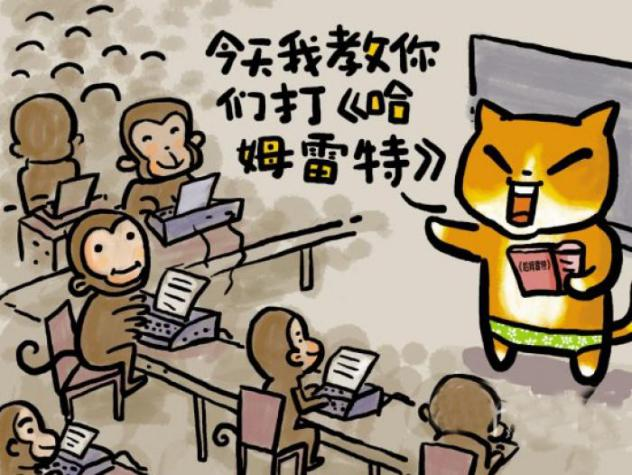
\includegraphics[]{img/Chapter8/8-12/1.png}
	\caption{无限猴子定理}
\end{figure}

这个看似不可能的事情,却可以用现有数学原理被推导出来。但在现实中往往被认为是无法实现的,因为人们认为“无限”这个条件通常无法被满足。根据概率论证,即使可观测宇宙中充满了猴子一直不停地打字,能够打出一部《哈姆雷特》的概率仍然小于$ 1 \over 10^{183900} $。\\

无限猴子定理同样可以用在排序中。如果给数组随机排列顺序,每一次排列之后验证数组是否有序,只要次数足够多,总有一次数组刚好被随机成有序数组。可是要想真的随机出有序数列,恐怕要等到猴年马月了。

\newpage